\documentclass[12pt]{article}

\usepackage{geometry}
\geometry{a4paper}

\usepackage{graphicx}
\graphicspath{{./resources/}}

% Used to import the Gannt chart
\usepackage{pdfpages}

% For Roman Numeral list
\usepackage{enumerate}

\usepackage{booktabs,longtable}

% For the Bibliography
\usepackage[english]{babel}
\usepackage[backend=bibtex]{biblatex}
\usepackage{csquotes}
\addbibresource{./bibliographies/agileSoftwareDevelopment}

\linespread{1.2}

\setlength{\parindent}{0pt}
\setlength{\parskip}{1em}

\begin{document}
	\begin{titlepage}
		\newcommand{\HRule}{\rule{\linewidth}{0.5mm}}
		
		\center
		
		\textsc{\LARGE Cardiff University}\\[1.5cm]
		\textsc{\Large Computer Science}\\[0.5cm]
		\textsc{\large CM2305: System's Design \& Group Project}\\[0.5cm]
		
		\HRule \\[0.4cm]
		\textsc{\Large \textbf{CAMEL}}\\[0.1cm]
		\textsc{\Large \textbf{CA}rdiff \textbf{M}athematics \textbf{E-L}earning}\\[0.7cm]
		{\huge\bfseries Agile Software Development}\\[0.4cm]
		\HRule \\[1.5cm]
		
		\begin{minipage}{0.4\textwidth}
			\begin{flushleft} \large
				\emph{Authors:}\\
				\mbox{Aimi \textsc{Nazihah}}
			\end{flushleft}
		\end{minipage}
		~
		\begin{minipage}{0.4\textwidth}
			\begin{flushright} \large
				\emph{Clients:} \\
				\mbox{Stuart \textsc{Allen}}, \mbox{Dafydd \textsc{Evans}}
			\end{flushright}
		\end{minipage}\\[3cm]
		
		{\large \today}\\[2cm]
		
		\vfill
	\end{titlepage}
	
	
	\tableofcontents
	
	\newpage
	
	\section{Project Management}
		There are a few software development methodologies in the software engineering field. For instance, Waterfall, Spiral and Agile. Even though Waterfall Model is popular version of the systems development life cycle as it rigid and linear, it may be not suitable for the CAMEL project because we are not building the system from scratch. This scenario is the same for Spiral Lifecycle Model as the model focuses on early identification and reduction of project risks as the system grows. So, we chose Agile Software Development with the justification in subsection below.
		
		\subsection{Agile Software Development}
			First and foremost, manifesto for Agile Software Development has laid out four values which are \cite{agileArtOfDevelopment}:
			
			\begin{enumerate}[i]
				\item \underline{Individuals and interaction} over processes and tools
				\item \underline{Working software} over comprehensive documentation
				\item \underline{Customer collaboration} over contract negotiation
				\item \underline{Responding to change} over following a plan
			\end{enumerate}
			
			These four values of Agile method are an environment that we are currently facing while working with the CAMEL project since our team members need to work together in terms of understanding and breaking the existing code. Since the existing prototype needs to be fixed, a working software is what we are aiming for. Along the way as we overhaul the existing codebase, client involvement is really crucial every now and then, to ensure the prototype is adhering to the requirements. Besides, our client is working together through the process of overhauling the existing code. Thus, we will respond to change and if our client has any changes to make, the requirements that we have agreed on will alter to the needs of the client.  
			
			Secondly, Agile has 12 Principles \cite{agileProjectManagementForDummies} that are a set of guiding concepts that support teams in implementing agile projects. One of the concepts says the most efficient and effective method to convey information to and within a development team is face-to-face conversation. We have planned to meet up at least once in a week for our group to study the existing code. Furthermore, learning code would need discussion and expertise from each and every one of us.
			
	\newpage
	
	\section{The Agile Roadmap to Value (Deliverables plan)}
		\begin{figure}[htbp]
			\centerline{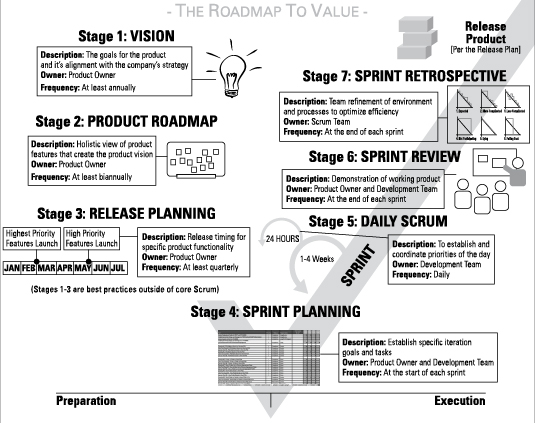
\includegraphics{roadmaptovalue.jpg}}
				\caption{Diagram 1: The Agile Roadmap to Value \cite{agileRoadmapToValue}}
		\end{figure}
		
		Diagram 1 shows The Roadmap to Value is a high level view of an agile project. We would use this roadmap following the term-time , which is from the first until last report and the prototype itself.
		
		In the first report, we have covered Stage 1, Stage 2 and Stage 3. The first stage we have identified the Product Vision that is briefly planned in the first section of report, which is System Requirements and Acceptance Criteria. In term of the frequency, we can change our planned task and deliverables whenever we need to. For second stage, since we have the existing codebase, even though it is not working right now, we already have the holistic view. Hence, we would improve the interface as we are working on the prototype. Next, in third stage, Table 1 below has described our Release Planning throughout the coursework timeline as a rough guide. 
		
		Apart from that, from Stage 4 until Stage 7 and the Product Release, we will explain in much more detail in accordance to our deliverables plan in Table 1.
		
		\label{table:agiledeliverablesplan}
		\setlength{\aboverulesep}{0pt}
		\setlength{\belowrulesep}{0pt}
		\begin{longtable}{|*{3}{p{3cm}|}}
			\toprule
			No. & Task & 1 \\
			\midrule
			\endfirsthead
			\multicolumn{3}{c}%
			{\tablename\ \thetable\ -- \textit{Continued from previous page}} \\
			\midrule
			No. & Task & 1 \\
			\midrule
			\endhead
			\hline \multicolumn{3}{r}{\textit{Continued on next page}} \\
			\endfoot
			\midrule
			\endlastfoot
			
			1 & Identify system requirements: functional and non-functional system requirements & 1 \\
			\midrule
			
			2 & Identify acceptance criteria: testable acceptance criteria associated with functional and non-functional requirements & 1 \\
			\midrule
			
			3 & Discussion of legal, social, ethical and professional issue & 1 \\
			\midrule
			
			4 & Do clear work plan, discuss a suitable software development process and state focus on next phase of project & 1 \\
			\midrule
			
			5 & Study existing code & 1 \\
			\midrule
			
			6 & Modify user interface (use navigation) & 2 \\
			\midrule
			
			7 & Design database and implication (including backup scheme) & 2 \\
			\midrule
			
			8 & Forms * & 2 \\
			\midrule
			
			9 & Provide exception handling & 2 \\
			\midrule
			
			10 & Provide error checking of end-user-input & 2 \\
			\midrule
			
			11 & Fix bugs on current system & 2 \\
			\midrule
			
			12 & Have maintainable code & 2 \& 3 \\
			\midrule
			
			13 & Admin and Developer documentation & 2 \& 3 \\
			\midrule
			
			14 & Testing framework  & 2 \& 3 \\
			\midrule
			
			15 & Allow logging of student answers to be compared later on & 2 \& 3 \\
			\midrule
			
			16 & Use the Python PEP8 coding convention & 2 \& 3 \\
			\midrule
			
			17 & Authors page (camel class \& how-to) & 3 \\
			\midrule
			
			18 & Break down teachers page & 3 \\
			\midrule
			
			19 & Add methods of checking and comparing student answers from questions & 3 \\
			\midrule
			
			20 & Add deadlines to student’s homework question  & 3 \\
			\midrule
			
			21 & Provide functionality to only see modules a student enrolled for & 3 \\
			\midrule
			
			22 & Ease of use & 3 \\
			\midrule
			
			23 & System should have security permissions to prevent unauthorised access to lecturer areas. & 3 \\
			\midrule
			
			\bottomrule
		\end{longtable}
		
		\textbf{Key:} *  -  high priority
		1st report: 27/11/15 – Initial Group \& Individual Report
		2nd report: 12/11/16 – Interim Group \& Individual Report
		3rd report: 29/11/16 – Final Group \& Individual Report \& Presentation
		
		The plan of deliverables table shows our aim to complete those tasks by respective reports. Since we are doing the task in pairs or individually, we may get started on high priority tasks and the others in parallel. At the end of the second deliverable, we expect to debug any errors which it initially had, and we will ensure testing of the prototype and ensure it has maintainable code following the standard. Apart from that, the tasks that we aimed to complete on the second and third report, it is more needed to ensure the maintainability to continue to the third report. For the third report, we aimed to complete all the tasks and expect the system working for all stakeholders; lecturers, authors, students and future developers. 
	
	\newpage
	
	\section{Extreme Programming}
		Extreme Programming is also featured as a part of the Agile Software Development approach \cite{agileModeling}. Extreme Programming (XP) is also a practice related with software development. I think it is suitable with the nature of our project because Extreme Programming stresses on customer satisfaction \cite{agileXPFlowchart}. Since our project is working closely with our client, our main aim is to have accomplished the requirements that we have agreed on.  It places a strong emphasis on technical practices in addition to the more common teamwork and structural practices \cite{agileArtOfDevelopment}.
		
		
		Apart from that, Extreme Programming emphasizes on teamwork as customers and developers are all in a collaborative team (Extreme Programming, n.d.) \cite{agileXPFlowchart}. It is meant to be implemented in a simple yet effective environment allowing teams to become highly productive. We as a team will also be self-organized to solve problems as efficiently as we can, such as trying to  work on priority tasks based on our capabilities.
		
		Starting on second deliverables and continuing into the third report, we aim to get feedback by testing the code on weekly basis. Each requirement that we succeed to implement will deepen unique contributions by each and every team member. 
		
		This diagram below shows overview of how XP works.  
		
		\begin{figure}[htbp]
			\centerline{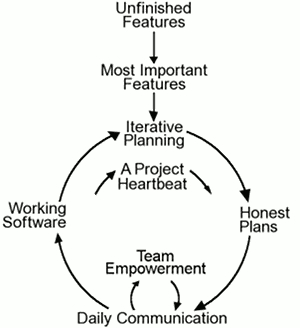
\includegraphics{agileflowchart.jpg}}
			\caption{Diagram 2: XP Flow chart \cite{agileXPFlowchart}}
		\end{figure}
		
		The flow of XP would compliment the situation we had, which is the existing code is an unfinished feature, then we need to identify any requirements that need to be prioritised. As time passes by, we will fulfil more requirements to enhance and improve the CAMEL system until it can be used for end users; students and lecturers.
	
	\newpage
	
	\section{First Group Report Gantt Chart}
		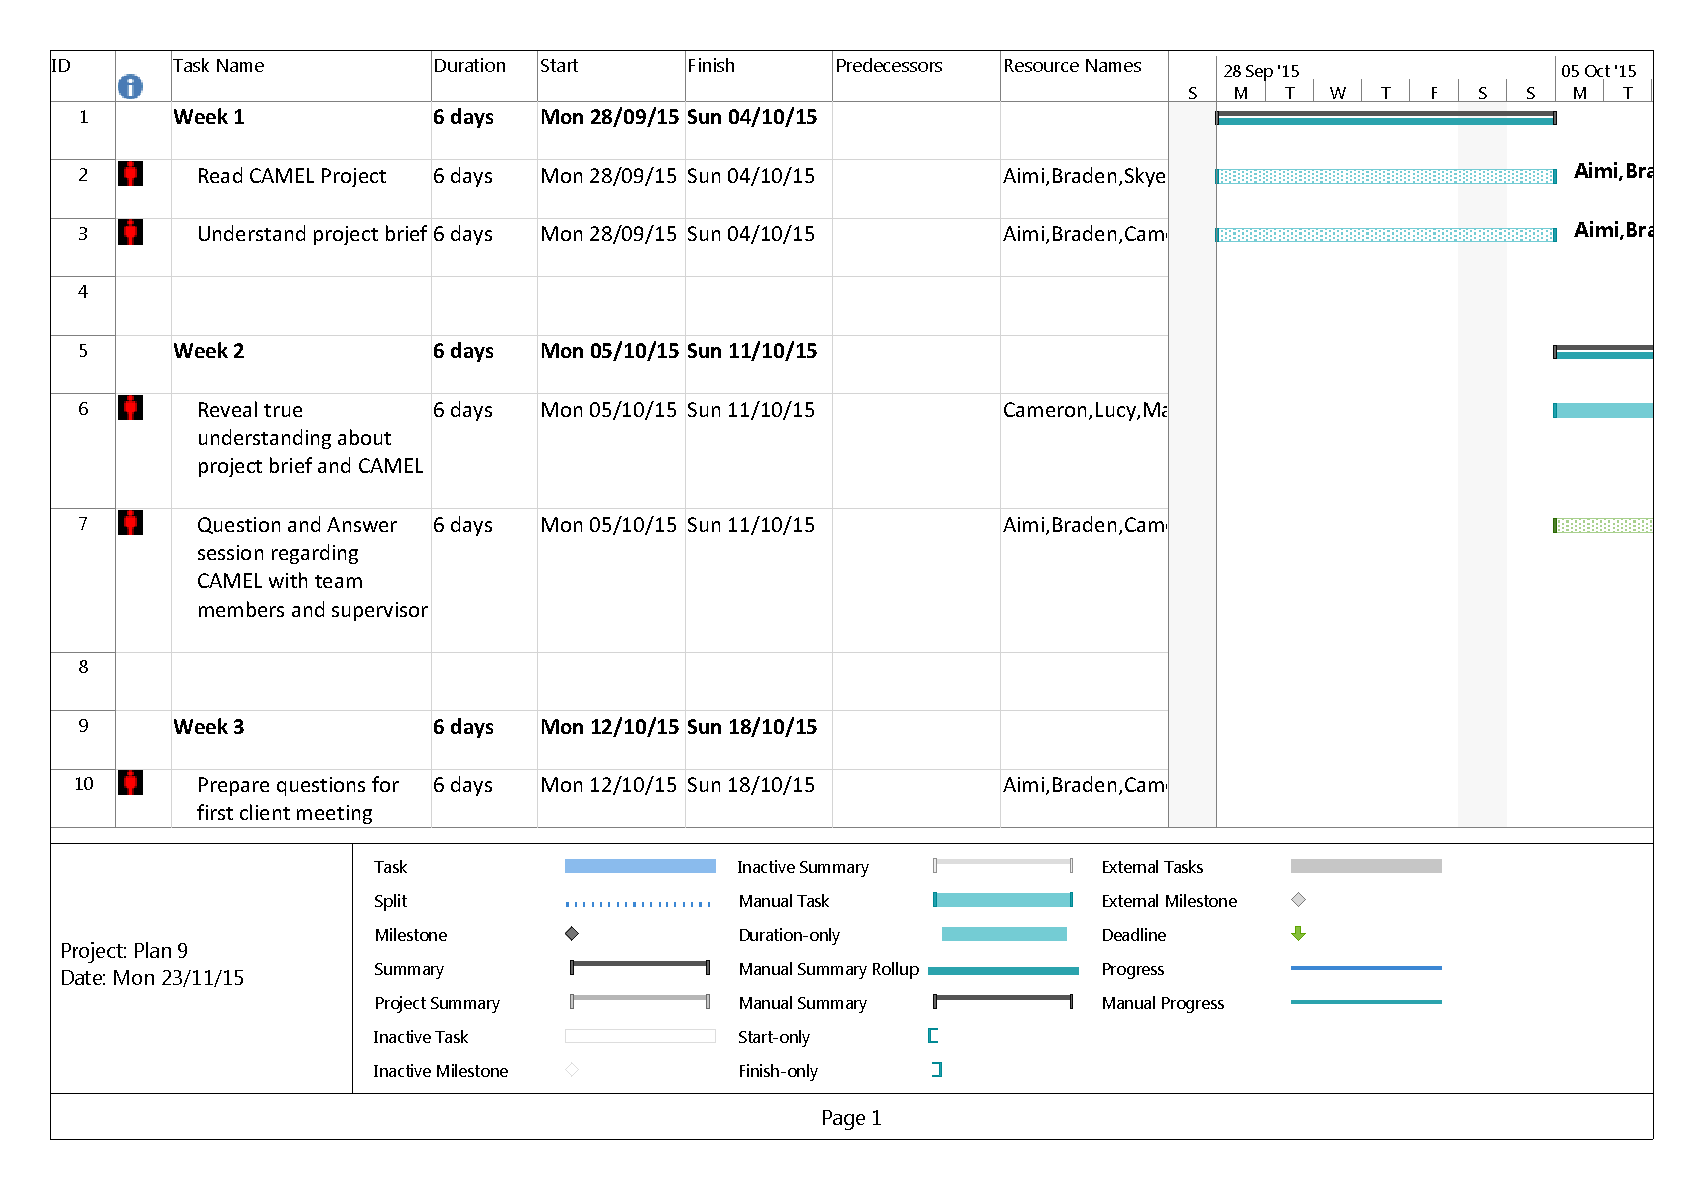
\includepdf[pages=-]{./resources/figureGanttChart.pdf}
		
	\newpage
	
	\section{Conclusion}
		The software development method we are going to use for working on the CAMEL system is Agile Software Development, and we will specifically be using the XP approach as it compliments the nature of our project. We will try to follow the deliverables as planned so that our client’s requirements are fulfilled. Last but not least, we aimed for a working end-system and maintainability for future development.
		
	\newpage
	
	\printbibliography
	
\end{document}
